\chapter{Turbulence Modelling} % Main chapter title
\label{Chapter2}

\section{Viscosity-Based Models}
Violeau et al. \parencite{VIOLEAU2002} were amongst the early pioneers who tried to incorporate a turbulence model in SPH. They came up with two techniques to tackle the problem of turbulence in a Lagrangian framework, which so far had been neglected till then in research, namely, the eddy viscosity model and a generalised Langevin model. For each of their techniques, they considered the following equation of state \ref{eq:violeau-eos}, continuity equation \ref{eq:violeau-continuity} and momentum equation \ref{eq:violeau-mom}, based on the work of \parencite{Monaghan1992}:

\begin{equation}
    P_i = B \Bigg[ \bigg( \frac{\rho_i}{\rho_0} \bigg)^{\gamma} - 1 \Bigg], B = \frac{\rho_0 c_s^2}{\gamma}
    \label{eq:violeau-eos}
\end{equation}
\begin{equation}
    \LagDerivative{\rho_i} = \sum_j m_j \VIJ \cdot \DWIJ
    \label{eq:violeau-continuity}
\end{equation}
\begin{equation}
    \LagDerivative{\vect{v}_i} = \sum_j m_j \bigg( \frac{P_i}{\rho_i^2} + \frac{P_j}{\rho_j^2} + \Pi_{ij} \bigg) \DWIJ + \vect{F}_i
    \label{eq:violeau-mom}
\end{equation}

Where the viscous term is defined as:
\begin{equation}
    \Pi_{ij} = - \frac{16\nu}{\rho_i + \rho_j} \frac{\VIJ \cdot \RIJ}{\RtwoIJ + \MachineEpsilon^2} 
    \label{eq:violeau-diffusion-term}
\end{equation}

\subsection{Eddy Viscosity Model}
\label{sec:eddy-visc-model}

The eddy viscosity model was devised as a first-order closure model, which consisted of a relationship between the Reynolds stress tensor and the mean velocity gradients. Therefore, the momentum equation is similar to the momentum equation, except that the kinematic viscosity is replaced by the eddy viscosity $(\nu_t)$, and the velocities are Reynolds-averaged. In the SPH formalism, the diffusion term occurring is therefore defined as given in \ref{eq:violeau-turbulent-diffusion-term}, with the eddy viscosity defined according to \ref{eq:violeau-eddy-viscosity}.
\begin{equation}
    \widetilde{\Pi}_{ij} = -8 \frac{\nu_{t, i} + \nu_{t, j}}{\rho_i + \rho_j} \frac{\RAProp{\vect{v}}_{ij} \cdot \RIJ }{\RtwoIJ + \MachineEpsilon^2}
    \label{eq:violeau-turbulent-diffusion-term}
\end{equation}
\begin{equation}
    \nu_t = L_m^2 \FrobeniusNorm{S} = L_m^2 \sqrt{\FrobeniusInnerProduct{S}{S}}
    \label{eq:violeau-eddy-viscosity}
\end{equation}

Where $\RAProp{\vect{v}}$ is Reynolds-averaged velocity, and $L_m$ refers to the mixing length scales. The SPH formulation for the mean velocity gradients are given in \ref{eq:violeau-mean-velocity-gradient}.

\begin{equation}
    \nabla \RAProp{\vect{v}}_i = - \frac{1}{\rho_i} \sum_j m_j \RAProp{\vect{v}}_{ij} \otimes \DWIJ
    \label{eq:violeau-mean-velocity-gradient}
\end{equation}

On simulating Poiseuille flow for a high Reynolds number case, the authors could show that the velocity profile showed only a slight discrepancy with theory, with the expected log-law profile near the walls \ref{fig:violeau2002-eddy-viscosity-result}. This indicated that the model is appropriate for turbulent mixing problems or for cases involving spatially-varying viscosity while restricted to shear flows.

\begin{figure}[h!]
    \centering
    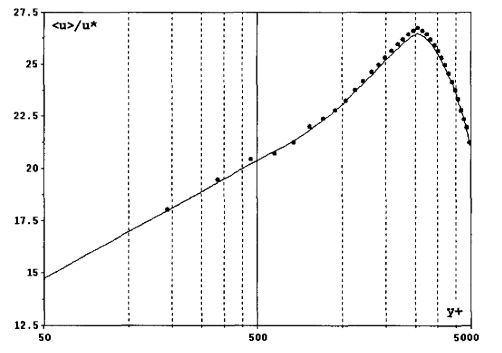
\includegraphics{Figures/research_papers/violeau2002-eddy-viscosity-result.png}
    \caption{Turbulent Poiseuille flow in a pipe $(Re = 64e3)$ modelled using the eddy viscosity model. Computed mean velocity profiles after $(t=1s)$ (solid circles), against theory (solid line). Ref: \parencite{VIOLEAU2002}}
    \label{fig:violeau2002-eddy-viscosity-result}
\end{figure}

\subsection{Generalized Langevin Model}
Violeau et al. also considered a stochastic approach, where the main idea is built on the concept of prescribing particle velocities as a random process, with properties fulfilling the theoretical turbulence hypotheses \parencite{pope1994lagrangi}. Hence, came about the Generalised Langevin model (GLM), where the particle acceleration is defined as:
\begin{equation}
    d\vect{v} = -\frac{1}{\rho} \nabla \RAProp{P} + \tensor{G}(\vect{v} - \RAProp{\vect{v}})dt + \sqrt{C_0 \epsilon dt}\vect{\xi}
    \label{eq:violeau-glm-particle-accel}
\end{equation}

Where $\Vec{\xi}$ is a random vector statistically non-correlated with velocities. The closure for this model was defined by specifying $\tensor{G}$ as:
\begin{equation}
    \tensor{G} = \HalfFrac C_1 \frac{\epsilon}{k}\tensor{I} + C_2 \nabla \RAProp{\vect{v}}
\end{equation}

Where $(k)$ is the turbulent kinetic energy, $(E)$ the dissipation rate, and $(C_i)$ being constants - $(C_1=1.8, C_2=0.6)$.
By modelling turbulence as GLM in SPH, the momentum equation derived was given by:
\begin{equation}
    \LagDerivative{\vect{v}_i} = -\sum_j m_j \bigg( \frac{\RAProp{P}_i}{\rho_i^2} + \frac{\RAProp{P}_j}{\rho_j^2} \bigg) \DWIJ - \HalfFrac C_1 \frac{\epsilon_i}{k_i} \vect{v}'_i + C_2 \nabla \RAProp{\vect{v}}_i \cdot \vect{v}'_i + \sqrt{\frac{C_0 \epsilon_i}{\delta t}} \Vec{\xi}_i
    \label{eq:violeau-mom-glm}
\end{equation}
\begin{equation}
    \RAProp{\vect{v}} = \sum_j \frac{m_j}{\rho_j}\vect{u}_j W_h (\vect{r}_j)
    \label{eq:violeau-ra-vel}
\end{equation}

Where the fluctuations are defined as $\vect{v}' = \vect{v} - \RAProp{\vect{v}}$, and the local values of turbulent kinetic energy and dissipation rate are:
\begin{align}
    \epsilon_i = 2 \nu_{t, i} + 
    \FrobeniusNorm{S_i}^2 \\
    k_i = \frac{\epsilon_i \nu_{t, i}}{C_{\mu}}, C_{\mu} = 0.009
    \label{eq:violeau-k-eps}
\end{align}

It is to be noted that the authors did not estimate the dissipation rate through the proper velocity gradients since the fluctuations of random velocities do not reproduce the small eddies.
The same test case as mentioned in \ref{sec:eddy-visc-model} was considered for the performance of GLM. 
The authors observed large fluctuations. They attributed the discrepancy to the mean operator being redefined as given by \ref{eq:violeau-ra-vel} instead of being a Reynolds average. In fact, by redefining the mean operator in such a fashion, they appeared to have constructed a rudimentary LES filter. 
As observed in \ref{fig:violeau2002-GLM-result}, the fluctuations have an order of magnitude of $k^{1/2}$. However, as claimed by the authors, unlike the eddy viscosity model, the GLM method can be used for different flows instead of being restricted to only shear flows.
\begin{figure}[h!]
    \centering
    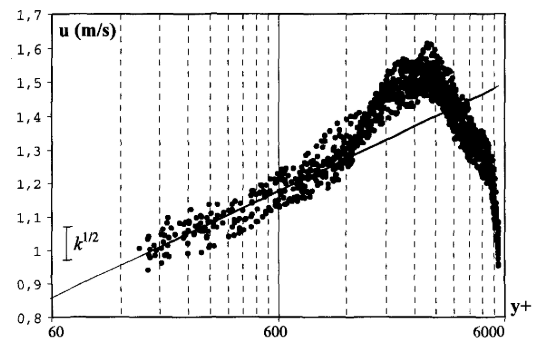
\includegraphics{Figures/research_papers/violeau2002-GLM-result.png}
    \caption{Turbulent Poiseuille flow in a pipe $(Re = 64e3)$ modelled using the generalised Langevin model. Computed mean velocity profiles after $(t=1s)$ (solid circles), against theory (solid line). Ref: \parencite{VIOLEAU2002}}
    \label{fig:violeau2002-GLM-result}
\end{figure}


\section{mSPH}
Adami et al. \parencite{Adami2012} devised a model built on their observation of SPH simulations, wherein the absence of viscosity in typical SPH formulations produced purely noisy particle motion. At finite viscosities, the method would over-predict dissipation. Hence to counter this, they essentially "modified" (hence the name: Modified SPH [mSPH]) the momentum equation and the equation of state to advect the particles in order to homogenise the particle distribution, in turn stabilising the numerical scheme. They were also able to reduce the artificial dissipation in transitional flows.

The authors considered summation density (\ref{eq:Adami2012-summation-density}), which is a function of the volume of the respective SPH particle as given by \ref{eq:Adami2012-vol}, as opposed to evolving density through the continuity equation \parencite{hu2006multi}. The modified equation of state as given by \ref{eq:Adami2012-eos}, is equivalent to the classical SPH equation-of-state with $\gamma=1$.
\begin{equation}
    \Vol_i = \frac{1}{\sum_j \WIJ}
    \label{eq:Adami2012-vol}
\end{equation}
\begin{equation}
    \rho_i = \frac{m_i}{\Vol_i} = m_i\sum_j \WIJ
    \label{eq:Adami2012-summation-density}
\end{equation}
\begin{equation}
    P_i = c_s^2 (\rho_i - \rho_0)
    \label{eq:Adami2012-eos}
\end{equation}

The momentum equation, which provides the acceleration of the particle, is a function of just the gradient and viscous shear forces as given by \ref{eq:Adami2012-mom-governing}. The corresponding SPH formulation was derived as given by \ref{eq:Adami2012-mom-sph}, which built on the earlier work of Hu and Adams \parencite{hu2007incompressible}.
\begin{equation}
    \LagDerivative{\vect{v}} = -\frac{1}{\rho}\nabla P + \nu \Delta( \vect{v} ) + \vect{F}
    \label{eq:Adami2012-mom-governing}
\end{equation}
\begin{equation}
    \LagDerivative{\vect{v}_i} = -\frac{1}{m_i} \sum_j (\Vol^2_i + \Vol^2_j) \frac{P_i \rho_j + P_j \rho_i}{\rho_i + \rho_i} \DWIJ - \frac{\eta}{m_i} \sum_j (\Vol^2_i + \Vol^2_j) \frac{\VIJ}{\RtwoIJ[]}\DWIJ + \vect{F}_i
    \label{eq:Adami2012-mom-sph}
\end{equation}

This scheme takes advantage of the regularisation of the
particle motion stemming from the additional background pressure $(P_0 = \rho_0 c_s^2)$. The additional force exerted by the background pressure counteracts non-homogeneous particle distributions, therein reducing numerical dissipation.

The authors estimated the energy spectra of the flow simulations in order to analyse the results of their test cases, using first and second-order moving-least-squares (MLS) method \parencite{gossler2001moving} and its subsequent Fourier transform \parencite{frigo2005design}.
Their first test case, the $2D$ variant of the Taylor-Green Vortex (TGV) problem, involved $8\times 8$ counter-rotating vortices, requiring $64^2$ particles. They considered the viscosity to be zero.
As seen in the time evolution of the 
\begin{figure}[h!]
    \centering
    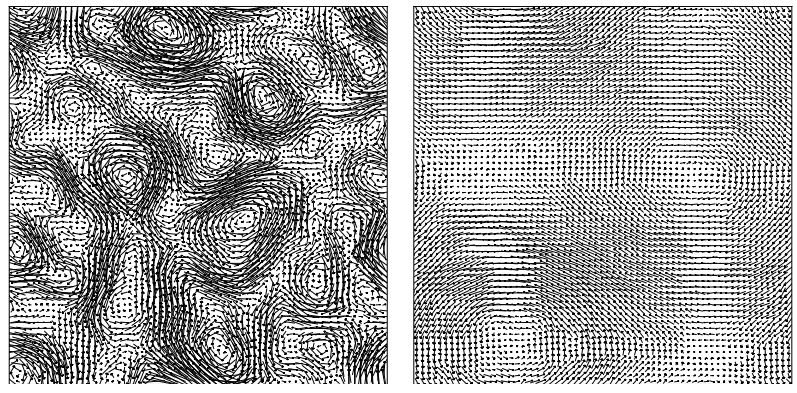
\includegraphics[scale=0.7]{Figures/research_papers/adami2012-evolution-vel-field-tgv.png}
    \caption{Velocity vector plot at $t=2$ (left) and $t=30$ (right). $Re = \infty$. Ref: \parencite{Adami2012} }
    \label{fig:adami2012-evolution-vel-field-tgv}
\end{figure}

The time evolution of the velocity field is given in \ref{fig:adami2012-evolution-vel-field-tgv}, where it can be observed that the $2D$ turbulence is characterised by merging and pairing of small vortices. The energy spectra given in \ref{fig:adami2012-energy-spectra-tgv} show that at low wave numbers, both interpolation schemes give the same results, but at high wave numbers, the results differ. The energy spectrum of the standard SPH has a linear slope of magnitude $m = 1$ in a log-log scale equivalent to a purely noisy velocity field. Theoretically, however, $2D$ turbulence has an energy cascade with a slope of $m = -3$ in the inertial range, which is reasonably predicted using mSPH.
\begin{figure}[h!]
    \centering
    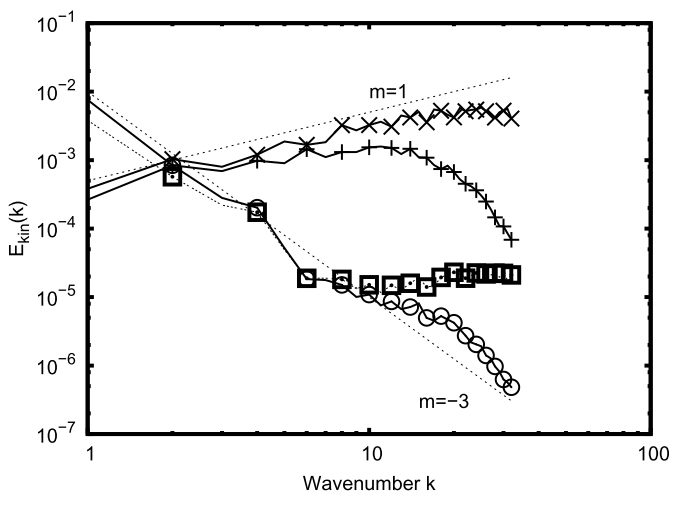
\includegraphics[scale=0.55]{Figures/research_papers/adami2012-energy-spectra-tgv.png}
    \caption{Comparison of energy spectra $t=10$. $+$ and $\times$ denote standard SPH results with quintic spline and MLS interpolation; $\circ$ and $\square$ denote mSPH results with quintic spline and MLS interpolation. Ref: \parencite{Adami2012} }
    \label{fig:adami2012-energy-spectra-tgv}
\end{figure}

The second test case employed by the authors was that of the $3D$ TGV problem requiring $64^3$ particles for a wide range of Reynolds numbers. The dissipation rate of the flow simulations are shown in \ref{fig:adami2012-dissipation-re400} and \ref{fig:adami2012-dissipation-re3000}. It can be observed that the standard SPH is unable to simulate transitional flows due to excessive dissipation. In contrast, mSPH can reproduce the dissipation rate reasonably well. This implies that the corrected particle transport velocity is an analogous eddy-viscosity model on scales below the numerical resolution.
\begin{figure}[h!]
    \centering
    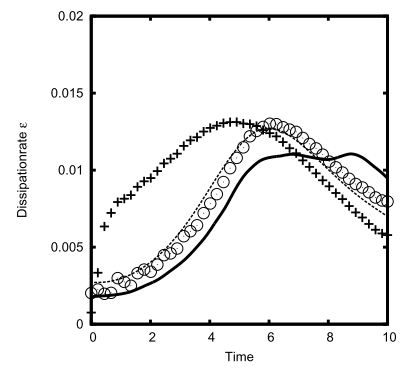
\includegraphics[scale=0.7]{Figures/research_papers/adami2012-dissipation-re400.png}
    \caption{Dissipation rate at $Re = 400$ using DNS (solid line), Smagorinsky model (dashed line), standard SPH ($+$) and mSPH ($\circ$). Ref: \parencite{Adami2012}}
    \label{fig:adami2012-dissipation-re400}
\end{figure}
\begin{figure}[h!]
    \centering
    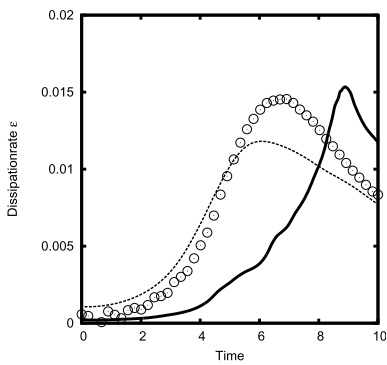
\includegraphics[scale=0.7]{Figures/research_papers/adami2012-dissipation-re3000.png}
    \caption{Dissipation rate at $Re = 3000$ using DNS (solid line), Smagorinsky model (dashed line) and mSPH ($\circ$). Ref: \parencite{Adami2012}}
    \label{fig:adami2012-dissipation-re3000}
\end{figure}

\section{Large Eddy Simulation-based Models}
\subsection{Implicit Pressure Poisson-based Models}
\label{sec:Implicit-Pressure-Poisson-based-Models}
Gotoh et al. \parencite{Gotoh2004} were amongst the first to integrate Large Eddy Simulation techniques with the SPH method. They derived this LES-SPH model, based on incompressible flow, to tackle the problem of reflection and transmission characteristics of regular waves by a partially immersed curtain-type breakwater. In order to compare the dissipation efficiencies, they considered the non-overtopping and overtopping cases of the problem.

The governing equations of the system were described as given by the continuity equation in \ref{eq:Gotoh2004-continuity-governing} and the momentum equation in \ref{eq:Adami2012-mom-governing}.
\begin{equation}
    \frac{1}{\rho} \LagDerivative{\rho} + \nabla \cdot \vect{v} = 0
    \label{eq:Gotoh2004-continuity-governing}
\end{equation}

The LES mass and momentum conservation equations for the flow were derived by filtering the respective equations using a spatial filter $\overline{(...)}$ to obtain their filtered counter-parts as given by \ref{eq:Gotoh2004-continuity-filtered} and \ref{eq:Gotoh2004-mom-filtered} respectively.
\begin{equation}
    \frac{1}{\rho} \LagDerivative{\rho} + \nabla \cdot \vect{\overline{v}} = 0
    \label{eq:Gotoh2004-continuity-filtered}
\end{equation}
\begin{equation}
    \LagDerivative{\vect{\overline{v}}} = -\frac{1}{\rho}\nabla \overline{P} + \nu \Delta ( \vect{\overline{v}} ) + \frac{1}{\rho}\nabla\cdot\tensor{\tau} + \vect{F}
    \label{eq:Gotoh2004-mom-filtered}
\end{equation}
\begin{equation}
    \frac{1}{\rho} \tensor{\tau} = \vect{\overline{v}} \otimes \vect{\overline{v}} - \overline{\vect{v} \otimes \vect{v}}
    \label{eq:Gotoh2004-stress-tensor}
\end{equation}

The stress tensor defined in \ref{eq:Gotoh2004-stress-tensor} is closed using Boussinesq's Hypothesis as defined in \ref{eq:Gotoh2004-boussinesq}.
\begin{equation}
    \frac{1}{\rho} \tensor{\tau} = 2\nu_t \tensor{S} - \frac{2}{3}k\tensor{I}
    \label{eq:Gotoh2004-boussinesq}
\end{equation}

The turbulent eddy viscosity is estimated using a modified Smagorinsky model as given in \ref{eq:Gotoh2004-eddy-visc}. This allows wall effects to be incorporated into the model, which the authors required to tackle the problem they were working on.
\begin{equation}
    \nu_t = \min(C_s \Delta x, \kappa d_{wall})^2 \sqrt{2 \FrobeniusInnerProduct{S}{S}}
    \label{eq:Gotoh2004-eddy-visc}
\end{equation}
\begin{equation}
    C_s=0.1, \kappa=0.4
\end{equation}

Where $(C_s)$ is the Smagorinsky constant, $(\kappa)$ is the von Karman constant and $d_{wall}$ is the normal distance of the particle to the closest wall.
The first term in \ref{eq:Gotoh2004-eddy-visc} dominates the flow far away from the solid wall, thereby recovering the standard Smagorinsky model. However, the second term dominates for flow close to the wall; hence, the eddy viscosity is a function of the particle distance to the wall. This overcomes the disadvantage of the standard Smagorinsky being over-dissipative inside the laminar layer.

In order to solve the system of equations and evolve them in time, the authors employed the Predictive-Corrective time integrator, similar to the two-step projection method of Chorin \parencite{chorin1968numerical}. The prediction stage is outlined by \ref{eq:Gotoh2004-predict-start} - \ref{eq:Gotoh2004-predict-end}. 
\begin{equation}
    \Delta \vect{v}_* = \bigg( \nu \Delta ( \vect{\overline{v}} ) + \frac{1}{\rho}\nabla\cdot\tensor{\tau} + \vect{F} \bigg) \Delta t
    \label{eq:Gotoh2004-predict-start}
\end{equation}
\begin{equation}
    \vect{v}_* = \vect{v}_t + \Delta \vect{v}_*
\end{equation}
\begin{equation}
    \vect{r}_* = \vect{r}_t + \vect{v}_* \Delta t
    \label{eq:Gotoh2004-predict-end}
\end{equation}

The correction stage is outlined by \ref{eq:Gotoh2004-correct-start} - \ref{eq:Gotoh2004-correct-end}. $(\overline{P})$ which is required to update the $(\vect{v}_{t+1})$ term is calculated implicitly from \ref{eq:Gotoh2004-correct-pressure-implicit}, which is based on the filtered continuity equation given by \ref{eq:Gotoh2004-continuity-filtered} and assuming incompressibility $\LagDerivative{\rho}=0$.
\begin{equation}
    \Delta \vect{v}_{**} = -\frac{1}{\rho} \nabla \overline{P}_{t+1} \Delta t
    \label{eq:Gotoh2004-correct-start}
\end{equation}
\begin{equation}
    \nabla \cdot \bigg( \frac{1}{\rho_*} \nabla \overline{P}_{t+1} \bigg) = \frac{\rho_0 - \rho_*}{\rho_0 \Delta t^2}
    \label{eq:Gotoh2004-correct-pressure-implicit}
\end{equation}
\begin{equation}
    \vect{v}_{t+1} = \vect{v}_* + \Delta \vect{v}_{**}
\end{equation}
\begin{equation}
    \vect{r}_{t+1} = \vect{r}_t + (\vect{v}_t + \vect{v}_{t+1})\frac{\Delta t}{2}
    \label{eq:Gotoh2004-correct-end}
\end{equation}

In order to solve the system of equations given by \ref{eq:Gotoh2004-predict-start} - \ref{eq:Gotoh2004-correct-end} in an SPH setting, the authors presented the following SPH formulation for the flow property. \textit{Note:} The over-line $\overline{(...)}$ convention used to denote filtered flow properties will be dropped in this sub-section unless stated otherwise.

The fluid density is given using a simple summation density \ref{eq:Gotoh2004-summation-density}.
\begin{equation}
    \rho_i = \sum_j m_j\WIJ
    \label{eq:Gotoh2004-summation-density}
\end{equation}

The pressure gradient term is defined in \ref{eq:Gotoh2004-grad-p-sph} in a symmetric form.
\begin{equation}
    \bigg( \frac{1}{\rho} \nabla P \bigg)_i = \sum_j m_j \bigg( \frac{P_i}{\rho_i^2} + \frac{P_j}{\rho_j^2} \bigg) \DWIJ
    \label{eq:Gotoh2004-grad-p-sph}
\end{equation}

The divergence of $\vect{v}$ is also defined symmetrically as given by \ref{eq:Gotoh2004-div-u-sph}.
\begin{equation}
    \nabla \cdot \vect{v}_i = \rho_i \sum_j m_j \bigg(\frac{\vect{v}_i}{\rho^2_i} + \frac{\vect{v}_j}{\rho^2_j} \bigg) \cdot \DWIJ
    \label{eq:Gotoh2004-div-u-sph}
\end{equation}

The pressure Laplacian, defined in \ref{eq:Gotoh2004-p-laplacian-sph}, is formulated as a hybrid of a standard SPH first derivative with a finite difference approximation for the first derivative to aid particle pressure stability \parencite{cummins1999sph}.
\begin{equation}
    \nabla \cdot \bigg( \frac{1}{\rho} \nabla P \bigg)_i = \sum_j m_j \frac{8}{(\rho_i + \rho_j)^2} \frac{P_{ij} \RIJ \cdot \DWIJ }{\RtwoIJ}
    \label{eq:Gotoh2004-p-laplacian-sph}
\end{equation}

The divergence of the stress tensor is defined in \ref{eq:Gotoh2004-div-tau-sph}.
\begin{equation}
    \bigg( \frac{1}{\rho} \nabla \cdot \tensor{\tau} \bigg)_i = \sum_j m_j \Bigg( \frac{1}{\rho_i^2}\tensor{\tau_i} + \frac{1}{\rho_j^2}\tensor{\tau_j} \Bigg) \cdot \DWIJ
    \label{eq:Gotoh2004-div-tau-sph}
\end{equation}

Finally, the laminar stress term, consisting of the velocity Laplacian term, is defined as given by \ref{eq:Gotoh2004-vel-laplacian-sph}.
\begin{equation}
    \big(\nu \Delta(\vect{v}) \big)_i = \sum_j m_j \frac{4(\eta_i + \eta_j)}{(\rho_i + \rho_j)^2}\frac{\VIJ \RIJ \cdot \DWIJ}{\RtwoIJ}
    \label{eq:Gotoh2004-vel-laplacian-sph}
\end{equation}

The authors used this SPH-LES model to investigate the wave interaction with a partially immersed breakwater and compared the results with experimentally obtained values of a similar setup. Their computational domain was $2D$ populated by $\approx 12e3$ particles.

\begin{figure}[h!]
    \centering
    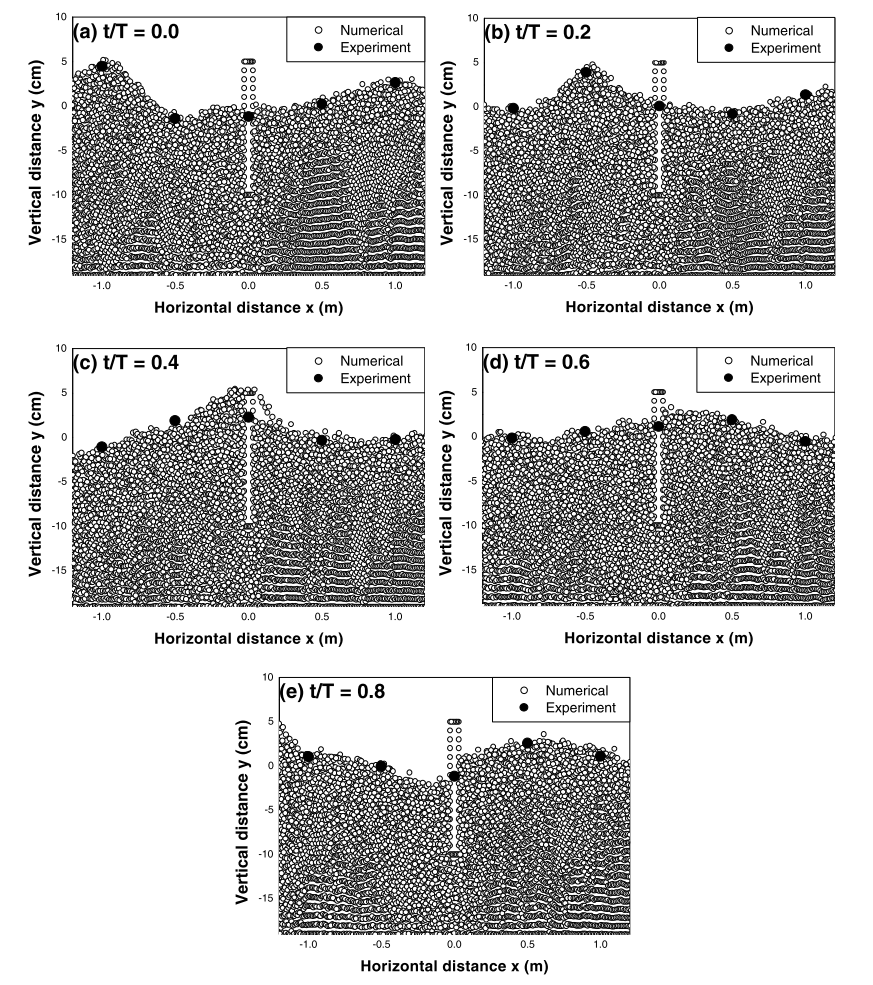
\includegraphics[scale=0.8]{Figures/research_papers/gotoh2004-wave-profile-result.png}
    \caption{Time sequences of computational and experimental wave profiles near curtain wall (overtopping). Ref: \parencite{Gotoh2004}}
    \label{fig:gotoh2004-wave-profile-result}
\end{figure}

As observed in the comparative plots given in \ref{fig:gotoh2004-wave-profile-result}, the model proves to be accurate in tracking free surfaces of large deformation without numerical diffusion. The authors also observed the model's capability to simulate turbulence and eddy vortices realistically near the curtain wall. However, the authors also conclude that a more refined turbulence model will be required for further accuracy in predicting flow involving wave interactions.

Building on the work mentioned above, Shao and Gotoh \parencite{Shao2005} performed a comparative study of SPH and the Moving Particle Semi-Implicit (MPS) method coupled with an LES model. They also validated these models against experimental data.

The filtered conservation equations which the authors considered were the same as given by \ref{eq:Gotoh2004-continuity-filtered} - \ref{eq:Gotoh2004-boussinesq}. However, they incorporated the standard Smagorinsky model \parencite{smagorinsky1963general} given by \ref{eq:Shao2005-eddy-visc} as opposed to the modified model \ref{eq:Gotoh2004-eddy-visc}.
\begin{equation}
    \nu_t = (C_s \Delta x)^2
    \label{eq:Shao2005-eddy-visc}
\end{equation}

The authors consider the same predictive-corrective scheme to evolve their system as detailed in \ref{eq:Gotoh2004-predict-start} - \ref{eq:Gotoh2004-correct-end}.
Similarly, they follow the same SPH formulation outlined in \ref{eq:Gotoh2004-summation-density} - \ref{eq:Gotoh2004-vel-laplacian-sph}. They do however, slightly modify the pressure and velocity Laplacian terms as given in \ref{eq:Shao2005-P-laplacian-sph} and \ref{eq:Shao2005-vel-laplacian-sph} respectively.
\begin{equation}
    (\nabla^2 P)_i = \sum_j m_j \frac{4}{\rho_i + \rho_j} \frac{P_{ij} \RIJ \cdot \DWIJ }{\RtwoIJ}
    \label{eq:Shao2005-P-laplacian-sph}
\end{equation}
\begin{equation}
    \big(\nu \Delta(\vect{v}) \big)_i = \sum_j m_j \frac{2(\nu_i + \nu_j)}{\rho_i + \rho_j}\frac{\VIJ \RIJ \cdot \DWIJ}{\RtwoIJ}
    \label{eq:Shao2005-vel-laplacian-sph}
\end{equation}

The authors validated this SPH-LES Model using experimental data from the experimental data corresponding to a solitary wave breaking on the beach \parencite{Synolakis1986}. Their computational domain was $2D$ and consisted of $\approx 18e3$ particles. 
From the computed wave profiles shown in \ref{fig:shao2005-wave-profile-result}, it can be visually observed that there is reasonable agreement between the experimental and computation data. This verifies the model's accuracy in tracking free surfaces with less or no numerical diffusion.
Furthermore, by performing a convergence study of the SPH-LES model using the dam-break problem, the authors could show that the scheme's spatial and temporal accuracy is $O(\Delta t + \Delta x^(1.25)$.

\begin{figure}[h!]
    \centering
    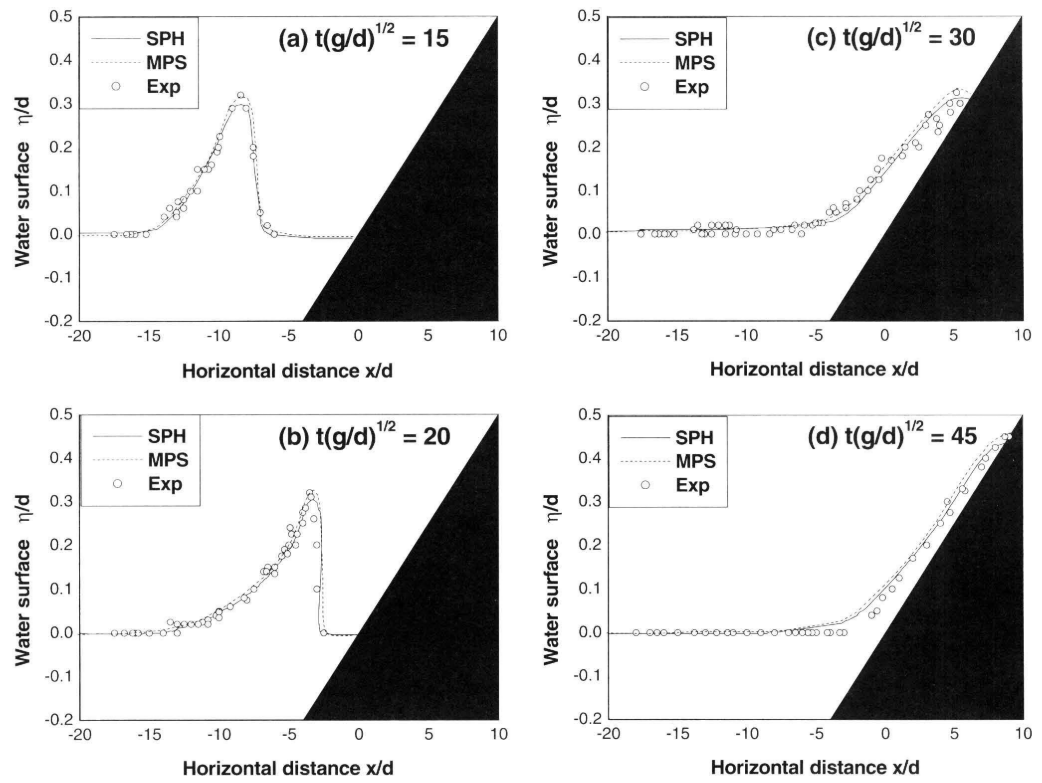
\includegraphics[scale=0.6]{Figures/research_papers/shao2005-wave-profile-result.png}
    \caption{Experimental and computational wave profiles by SPH and MPS model. Ref: \parencite{Shao2005}}
    \label{fig:shao2005-wave-profile-result}
\end{figure}


\subsection{Explicit Pressure Equation of State-based Solvers}
\subsubsection{Standard Smagorinsky Model}

Rogers and Dalrymple \parencite{ROGERS2005}, similar to the work on SPH-LES modelling detailed in \ref{sec:Implicit-Pressure-Poisson-based-Models}, came up with an LES-type sub-particle-scale (SPS) formulation based on the weakly compressible assumption in order to develop a turbulence model for SPH.

The authors considered the mass and momentum conservation equations as already given in \ref{eq:Gotoh2004-continuity-governing} and  \ref{eq:Adami2012-mom-governing} respectively, along with the equation of state \ref{eq:violeau-eos}. However, for the value of $(B)$ in the state equation, the authors considered the definition given in \ref{eq:ROGERS2005-eos-b}:
\begin{equation}
    B = 10 u_{max}
    \label{eq:ROGERS2005-eos-b}
\end{equation}

They subsequently filtered the compressible conservation equations using Favre averaging as given by \ref{eq:ROGERS2005-favre-averaging}.
\begin{equation}
    \widetilde{f} = \frac{\overline{\rho f}}{\overline{\rho}}
    \label{eq:ROGERS2005-favre-averaging}
\end{equation}

The derived filtered conservation equations for mass and momentum are detailed in \ref{eq:ROGERS2005-continuity-filtered} and \ref{eq:ROGERS2005-mom-filtered}.
\begin{equation}
    \LagDerivative{\overline{\rho}} = -\overline{\rho} \nabla \cdot \vect{\widetilde{v}}
    \label{eq:ROGERS2005-continuity-filtered}
\end{equation}
\begin{equation}
    \LagDerivative{\vect{\widetilde{v}}} = - \frac{1}{\overline{\rho}}\nabla \overline{P} + \frac{1}{\overline{\rho}} (\nabla \cdot \overline{\rho \nu} \nabla) \vect{\widetilde{v}} + \frac{1}{\overline{\rho}}\nabla\cdot\tensor{\tau} + \vect{F}
    \label{eq:ROGERS2005-mom-filtered}
\end{equation}

Where the SPS stress tensor and turbulent eddy viscosity is given by \ref{eq:ROGERS2005-tau} and \ref{eq:ROGERS2005-turbulent-eddy-visc} respectively.
\begin{equation}
    \tensor{\tau} = \overline{\rho}\bigg(2\nu_t \tensor{S} - \frac{2}{3}\operatorname{tr}[\tensor{S}]\tensor{I}\bigg) - \frac{2}{3}\overline{\rho}C_I \overline{\Delta}^2 \tensor{I}, C_I = 6.6e-4
    \label{eq:ROGERS2005-tau}
\end{equation}
\begin{equation}
    \nu_t = (C_s \Delta x)^2 \sqrt{2 \FrobeniusInnerProduct{S}{S}}, C_s = 0.12
    \label{eq:ROGERS2005-turbulent-eddy-visc}
\end{equation}

As for the SPH formulations of the aforementioned governing equations, the authors

The authors derived the SPH formulations of the aforementioned governing equations. The continuity equation takes the form as detailed in \ref{eq:violeau-continuity}. The pressure gradient term is given in \ref{eq:Gotoh2004-grad-p-sph}. The laminar stress term, consisting of the velocity Laplacian is given by \ref{eq:ROGERS2005-vel-laplacian-sph}, which itself was built on the work of Morris et al. \parencite{morris1997modeling} as given in \ref{eq:morris1997modeling-vel-laplacian-sph}. Finally the stress divergence is defined by \ref{eq:Gotoh2004-div-tau-sph}.
\begin{equation}
    \bigg( \frac{1}{\rho} (\nabla \cdot \eta \nabla) \vect{v} \bigg)_i = \sum_j m_j \frac{\nu (\rho_i + \rho_i)}{\rho_{ij}^2} \frac{\VIJ \RIJ \cdot \DWIJ}{\RtwoIJ + \MachineEpsilon}
    \label{eq:ROGERS2005-vel-laplacian-sph}
\end{equation}
\begin{equation}
    \bigg( \frac{1}{\rho} (\nabla \cdot \eta \nabla) \vect{v} \bigg)_i = \sum_j m_j \frac{(\eta_i + \eta_j) \VIJ}{\rho_i \rho_j} \bigg( \frac{1}{\RtwoIJ[]} \PartialDerivative[r_i]{\WIJ} \bigg), \DWIJ = \frac{\RIJ}{\RtwoIJ[]} \PartialDerivative[r_i]{\WIJ}
    \label{eq:morris1997modeling-vel-laplacian-sph}
\end{equation}

The authors noted that the LES description of viscous effects in
slightly compressible SPH could lead to unphysical behaviour at free surfaces due to density variations being magnified by the equation of state. The lack of artificial viscosity implies that such variations are not damped. They subsequently noted that averaging the density would ensure smooth and physically acceptable free surfaces, based on the work of Panizzo \parencite{panizzo2004physical}. Hence, they performed Shepard filtering of the density as defined in \ref{eq:ROGERS2005-rho-shepard-filter} every 40-time steps.
\begin{equation}
    \rho_i = \frac{\sum_j \rho_j \WIJ \Vol_j}{\sum_j \WIJ \Vol_j}
    \label{eq:ROGERS2005-rho-shepard-filter}
\end{equation}

The authors simulated the problem of a weakly plunging breaker in $2D$ and $3D$ to ascertain the performance and capability of the model. Their $2D$ computational domain consisted of $\approx 1e5$ particles, with the $3D$ domain consisting $\approx 2e4$ particles.
The authors were able to show that in the case of the $2D$ problem, the model could predict regions of high vorticity that persisted longer when compared to standard SPH utilising conventional artificial viscosity. The model also displayed the turbulent bore, which generated reverse breaking, leading to the downbursting-like phenomenon, as observed in experiments \parencite{kubo2001large}.
In the case of the $3D$ problem, the authors showed the model's capability to capture near vertically-oriented eddies despite the lower resolution. 

Building on this work, Dalrymple and Rogers \parencite{Dalrymple2006} used this scheme on a wide variety of problems, ranging from $2D$ Green water overtopping, $2D$ waves on a beach, $3D$ dam break and $3D$ waves on a beach. The quantitative analysis of the results allowed the authors to conclude that the model is especially suited for problems involving splash or flow separation. The authors also warn about the model's requirement of a large number of particles for sufficient resolution. That and the finite speed of sound stemming from the compressible flow implied that time steps had to $O(10^{-5}s)$. Hence, the authors remain cautiously optimistic about the model since the method performs well for smaller regions where the number of particles is reasonable. However, they believe that extended Boussinesq codes would more efficiently model larger domains.

\subsubsection{Modified Smagorinsky Model}
Canelas et al. \parencite{Canelas2016} constructed the wall-adapting local eddy viscosity (WALE) model to be incorporated in the SPH-LES scheme. They noted that studying turbulent flow fields required the identification of vortices themselves to study their interactions in the flow. They used the definition of Lagrangian Coherent Structures (LCS) to help capture these vortices. As a Lagrangian method, SPH is preferable for the study of LCS since the technique provides the motion of individual fluid particles, thereby eliminating the need for expensive post-processing inherent to Eulerian solutions. 
However, they noted that typically employed SPS strategies for LES simulations, based on the standard Smagorinsky model, cannot correctly enforce wall conditions and non-vanishing stresses with laminar flows. Hence they devised the WALE model.

The authors consider the compressible Navier-Stokes along the continuity equation as their governing equation. They subsequently present the SPH formulation of the continuity equation as defined by \ref{eq:Canelas2016-continuity-sph}.
\begin{equation}
    \LagDerivative{\rho_i} = - \rho_i \sum_j m_j \VIJ \cdot \DWIJ
    \label{eq:Canelas2016-continuity-sph}
\end{equation}
The pressure gradient term is given in \ref{eq:Gotoh2004-grad-p-sph}. The laminar stress term, consisting of the velocity Laplacian, is given by \ref{eq:Canelas2016-vel-laplacian-sph}. 
\begin{equation}
    \big(\nu \Delta(\vect{v}) \big)_i = \sum_j m_j \frac{4 \nu}{\rho_i + \rho_j}\frac{\VIJ \RIJ \cdot \DWIJ}{\RtwoIJ}
    \label{eq:Canelas2016-vel-laplacian-sph}
\end{equation}

Finally the stress divergence is defined by \ref{eq:Gotoh2004-div-tau-sph}, with the stress tensor being defined by \ref{eq:Canelas2016-tau}
\begin{equation}
    \tensor{\tau} = \rho \bigg( 2\nu_t \tensor{S} - \frac{2 \nu_t}{3}\operatorname{tr}[\tensor{S}]\tensor{I} \bigg) - \frac{4}{3} \rho C_I \Delta^2 \tensor{I} \FrobeniusInnerProduct{S}{S}, C_I = 6.6e-3
    \label{eq:Canelas2016-tau}
\end{equation}

The WALE model redefines the turbulent eddy viscosity as given by \ref{eq:Canelas2016-turbulent-eddy-visc}.
\begin{equation}
    \nu_t = \rho (C_w \Delta x)^2 \frac{\FrobeniusInnerProduct{S^d}{S^d}^{3/2}}{\FrobeniusInnerProduct{S}{S}^{5/2} + \FrobeniusInnerProduct{S^d}{S^d}^{5/4}}, C_w=0.325
    \label{eq:Canelas2016-turbulent-eddy-visc}
\end{equation}
Where
\begin{equation}
    \tensor{S^d} = \HalfFrac \bigg( (\nabla \vect{v})^2 + \big((\nabla \vect{v})^T\big)^2 \bigg) - \frac{1}{3} \operatorname{tr}[(\nabla \vect{v})^2] \tensor{I}
\end{equation}

In order to test their model, the authors considered an array of cylinders in fluid flow as shown in \ref{fig:Canelas2016-vel-field}, with a constant body force. They computed the vorticity field and the Finite-Time Lyapunov Exponents (FTLE) field to study the LCSs in the flow. These fields are shown in \ref{fig:Canelas2016-vorticity-field} and \ref{fig:Canelas2016-ftle-field} respectively.
 \begin{figure}[h!]
    \centering
    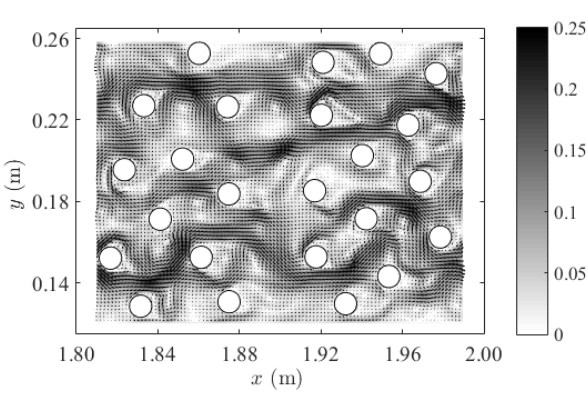
\includegraphics{Figures/research_papers/Canelas2016-vel-field.png}
    \caption{Cylinder distribution and instantaneous velocity overlapped by velocity vectors. Velocity in $m/s$, at $t=20s$. The flow direction is from left to right. Ref: \parencite{Canelas2016}}
    \label{fig:Canelas2016-vel-field}
\end{figure}
\begin{figure}[h!]
    \centering
    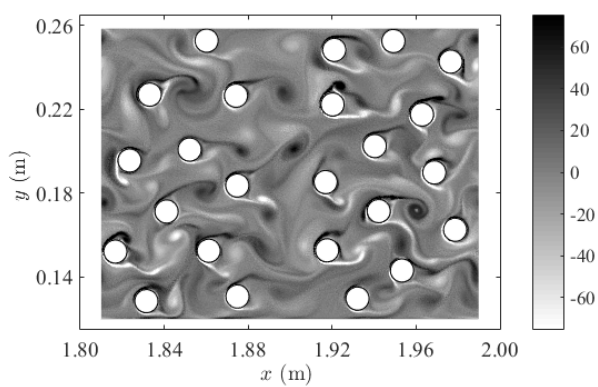
\includegraphics{Figures/research_papers/Canelas2016-vorticity-field.png}
    \caption{Vorticity field. Vorticity in Hz, at $t = 20s$. Ref: \parencite{Canelas2016}}
    \label{fig:Canelas2016-vorticity-field}
\end{figure}
\begin{figure}[h!]
    \centering
    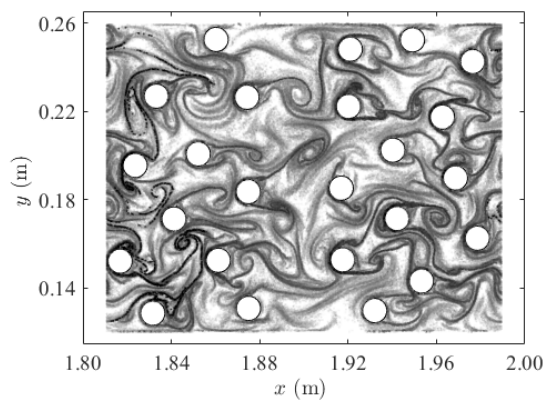
\includegraphics{Figures/research_papers/Canelas2016-ftle-field.png}
    \caption{FTLE field with negative integration time $(T = -0.4 s)$ (unstable manifolds - attracting LCS) at $t = 20s$. Ref: \parencite{Canelas2016}}
    \label{fig:Canelas2016-ftle-field}
\end{figure}

\subsection{Quasi-Lagrangian Models}

\subsection{RANS-based $k-\epsilon$ Models}

Shao \parencite{Shao2006} demonstrated that the two-equation $k-\epsilon$ model, an extensively studied model derived from the Reynolds-averaged Navier–Stokes (RANS) equations, can be incorporated in the truly incompressible version of SPH (ISPH). By attempting to extend RANS equations, which are hugely successful in practical fields, to a mesh-free method such as SPH, the author provides a framework to build on the wide variety of closure models available.

To discretise the RANS equations to an SPH form, the author considers the Reynolds averaged mass and momentum conservation equations as given in \ref{eq:Shao2006-rans-continuity-governing} and \ref{eq:Shao2006-rans-mom-governing} respectively. \textit{Note:} The averaged flow properties are represented without any over-line $\overline{(...)}$ hereafter.
\begin{equation}
    \frac{1}{\rho} \LagDerivative{\rho} + \nabla \cdot \vect{v} = 0, \LagDerivative{\rho} = 0 \text{ (Incompressible)}
    \label{eq:Shao2006-rans-continuity-governing}
\end{equation}
\begin{equation}
    \LagDerivative{\vect{v}} = -\frac{1}{\rho}\nabla P + \nu \Delta( \vect{v} ) + \frac{1}{\rho} \nabla \cdot \tensor{\tau} + \vect{F}
    \label{eq:Shao2006-rans-mom-governing}
\end{equation}

The stress tensor is given by \ref{eq:Gotoh2004-boussinesq}, while the turbulent eddy viscosity is defined as \ref{eq:Shao2006-turbulent-eddy-visc}.
\begin{equation}
    \nu_t = c_d \frac{k^2}{\epsilon}
    \label{eq:Shao2006-turbulent-eddy-visc}
\end{equation}

The transport equations for the turbulent kinetic energy and dissipation rate is given by \ref{eq:Shao2006-k-transport-eq} and \ref{eq:Shao2006-eps-transport-eq} respectively.
\begin{equation}
    \LagDerivative{k} = \nabla \cdot \bigg( \frac{\nu_t}{\sigma_k} \nabla k \bigg) + P_k - \epsilon
    \label{eq:Shao2006-k-transport-eq}
\end{equation}
\begin{equation}
    \LagDerivative{\epsilon} = \nabla \cdot \bigg( \frac{\nu_t}{\sigma_{\epsilon}} \nabla \epsilon \bigg) + c_{1\epsilon} \frac{\epsilon}{k} P_k - c_{2\epsilon} \frac{\epsilon^2}{k}
    \label{eq:Shao2006-eps-transport-eq}
\end{equation}
\begin{equation}
    P_k = 2\nu_t \FrobeniusInnerProduct{S}{S}
    \label{eq:Shao2006-k-production-term}
\end{equation}

Where, $(\sigma_k, \sigma_{\epsilon}, c_{1\epsilon}, c_{2\epsilon}) = (1.0, 1.3, 1.44, 1.92)$ are empirical constants dependent on the nature of the flow , and $(P_k)$ is the turbulence production rate, which satisfies the relation given by \ref{eq:pope2000turbulent-k-production-relation} \parencite{pope2000turbulent}.
\begin{equation}
    \frac{P_k}{\epsilon} = c_d \Bigg( \frac{\sqrt{2 \FrobeniusInnerProduct{S}{S}}}{\epsilon} \Bigg)
    \label{eq:pope2000turbulent-k-production-relation}
\end{equation}

These governing equations are solved and evolved using the same predictive-corrective time integrator as seen in the work of \parencite{Gotoh2004}, and outlined in \ref{eq:Gotoh2004-predict-start} - \ref{eq:Gotoh2004-correct-end}.

As for the SPH formulations of the governing equations, the author builds on the work of \parencite{Gotoh2004}, and uses the same discretization as defined in \ref{eq:Gotoh2004-summation-density} - \ref{eq:Gotoh2004-div-tau-sph}. However, the author uses a slightly modified version of the laminar stress term given in \ref{eq:Gotoh2004-vel-laplacian-sph} and redefines it as given in \ref{eq:Shao2006-vel-laplacian-sph}.
\begin{equation}
    \big(\nu \Delta(\vect{v}) \big)_i = \sum_j m_j \frac{2 ( \nu_i + \nu_j ) }{ \rho_i + \rho_j }\frac{\VIJ \RIJ \cdot \DWIJ}{\RtwoIJ}
    \label{eq:Shao2006-vel-laplacian-sph}
\end{equation}

The author tested the model on the problem of $2D$ wave breaking and overtopping of a sloping wall and compared the results obtained against experimental data \parencite{li2004wave} to validate the model—the computational domain of $\approx 6e3$ particles.

As seen from the evolution of the water surface elevation plotted in \ref{fig:Shao2006-water-surf-elevations}, the author could ascertain that the proposed model produced better results than those of Li et al. \parencite{li2004wave}, compared to the experimental data in \ref{fig:Shao2006-water-surf-elevations}(a) and \ref{fig:Shao2006-water-surf-elevations}(b). This could be attributed to the free surfaces being accurately tracked by particles without numerical diffusion. 
In \ref{fig:Shao2006-water-surf-elevations}(c) and \ref{fig:Shao2006-water-surf-elevations}(d), despite the wave profiles being consistent with each other in phase and shape, the proposed model predicts smaller elevation levels. Li et al. use a dynamic Smagorinsky model, whereas the proposed model uses constant empirical coefficients. The author believes these coefficients derived from a quasi-steady state may behave sub-optimally in transient flow, such as the problem at hand.
\begin{figure}[h!]
    \centering
    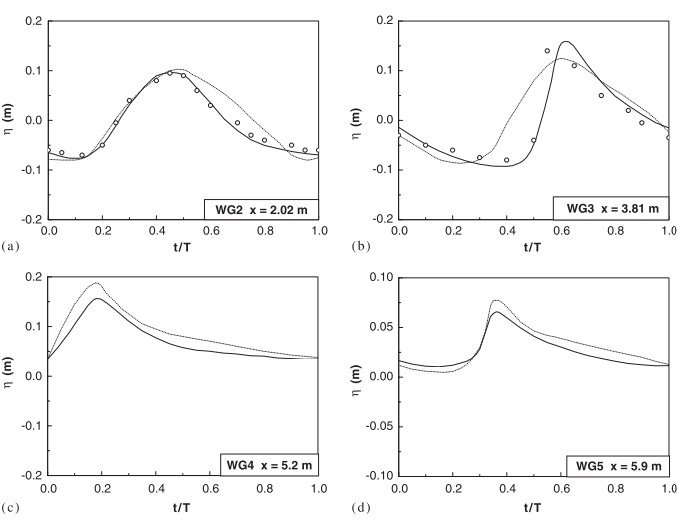
\includegraphics[scale=0.9]{Figures/research_papers/Shao2006-water-surf-elevations.png}
    \caption{Comparisons of computed water surface elevations by SPH (solid lines) with experimental ($\circ$) and numerical (dotted lines) data of Li et al. \parencite{li2004wave}. Ref: \parencite{Shao2006}}
    \label{fig:Shao2006-water-surf-elevations}
\end{figure}

The author concludes that the $k-\epsilon$ model would require further sensitivity analysis for the turbulence model and spatial resolution for improved results, despite being reasonably accurate in tracking free surfaces.

Wang and Liu \parencite{Wang2020} build on the work of Shao \parencite{Shao2006} to further improve the ISPH $k-\epsilon$ model. They achieved this by using the modelling and computational developments which SPH has benefited from since the work of Shao.
The authors here consider the same SPH discretised equations and two-step time integrator as Shao, with two distinct modifications in the Pressure Poisson equation as given by \ref{eq:Wang2020-correct-pressure-implicit} instead of \ref{eq:Gotoh2004-correct-pressure-implicit}. They also redefined propagation equation for $(\vect{r}$ using \ref{eq:Wang2020-correct-end} instead of \ref{eq:Gotoh2004-correct-end}.
\begin{equation}
    \nabla \cdot \bigg( \frac{1}{\rho_0} \nabla P_{t+1} \bigg) = \frac{1}{\Delta t} \nabla \cdot \vect{u_*}
    \label{eq:Wang2020-correct-pressure-implicit}
\end{equation}
\begin{equation}
    \vect{r}_{t+1} = \vect{r}_* + \Delta \vect{v}_{**} \Delta t
    \label{eq:Wang2020-correct-end}
\end{equation}

The authors also provided SPH discretization for the transport equations for $(k)$ and $(\epsilon)$ using \ref{eq:Wang2020-k-laplacian} and \ref{eq:Wang2020-eps-laplacian} which requires the use of particle density $(\varphi)$ as given in \ref{eq:Wang2020-particle-density}.
\begin{equation}
    \varphi_i = \sum_j \WIJ
    \label{eq:Wang2020-particle-density}
\end{equation}
\begin{equation}
    \nabla \cdot \bigg( \frac{\nu_t}{\sigma_k} \nabla k \bigg)_i = - \sum_j \frac{1}{\varphi_j} \bigg( \frac{\nu_{t,i}}{\sigma_k} + \frac{\nu_{t,i}}{\sigma_k}  \bigg) \frac{k_{ij} \RIJ \DWIJ}{\RtwoIJ}
    \label{eq:Wang2020-k-laplacian}
\end{equation}
\begin{equation}
    \nabla \cdot \bigg( \frac{\nu_t}{\sigma_{\epsilon}} \nabla \epsilon \bigg)_i = - \sum_j \frac{1}{\varphi_j} \bigg( \frac{\nu_{t,i}}{\sigma_{\epsilon}} + \frac{\nu_{t,i}}{\sigma_{\epsilon}}  \bigg) \frac{\epsilon_{ij} \RIJ \DWIJ}{\RtwoIJ}
    \label{eq:Wang2020-eps-laplacian}
\end{equation}

The authors also derived an SPH formulation for the strain rate tensor defined in \ref{eq:Wang2020-strain-rate-tensor}, which is based on the studies done on kernel correction \parencite{bonet1999variational, khayyer2008corrected} and given by \ref{eq:Wang2020-vel-grad-term} and \ref{eq:Wang2020-corrective-matrix}. 
\begin{equation}
    \tensor{S}_i = \HalfFrac \bigg( \nabla \vect{v}_i + (\nabla \vect{v}_i)^T \bigg)
    \label{eq:Wang2020-strain-rate-tensor}
\end{equation}
\begin{equation}
    \nabla \vect{v}_i = - \sum_j \frac{1}{\varphi_j} \VIJ \otimes \tensor{L}_i \DWIJ
    \label{eq:Wang2020-vel-grad-term}
\end{equation}
\begin{equation}
    \tensor{L}_i = \Bigg(- \sum_j \frac{1}{\varphi_j} \DWIJ \otimes \RIJ \Bigg)^{-1}
    \label{eq:Wang2020-corrective-matrix}
\end{equation}

The authors validated the model against the problem of a solitary wave propagating over a bottom-mounted barrier in $2D$. Its results are shown in \ref{fig:Wang2020-wave-propogation-result}. They also considered the problem involving wave breaking on a slopping wall in $2D$, which is shown in \ref{fig:Wang2020-wave-breaking-result}.
\begin{figure}[h!]
    \centering
    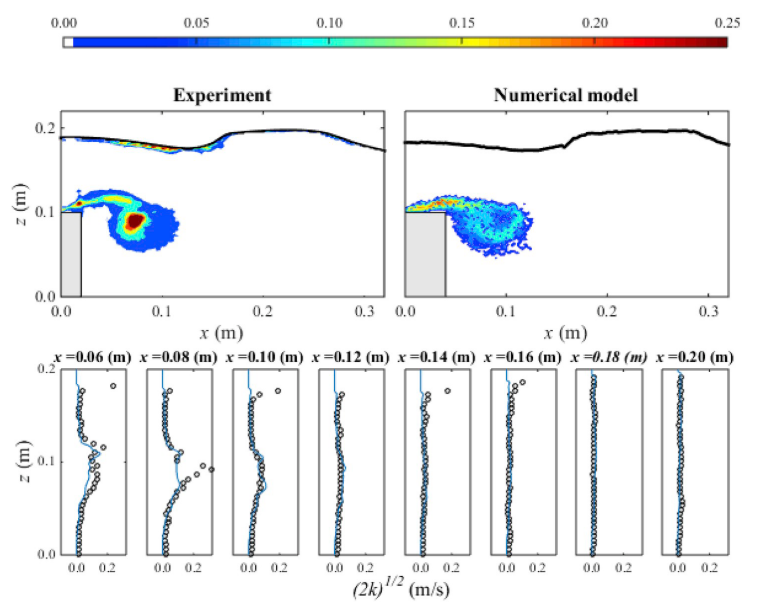
\includegraphics[scale=0.75]{Figures/research_papers/Wang2020-wave-propogation-result.png}
    \caption{Comparisons between experimental data (left) and numerical results (right) for turbulence intensity $(m/s)$ at $t=0.6s$ (top panels) and the corresponding vertical cross-sections (lower panels). In the lower panels, solid lines and $\circ$ represent the numerical and experimental results, respectively. Ref: \parencite{Wang2020}}
    \label{fig:Wang2020-wave-propogation-result}
\end{figure}
\begin{figure}[h!]
    \centering
    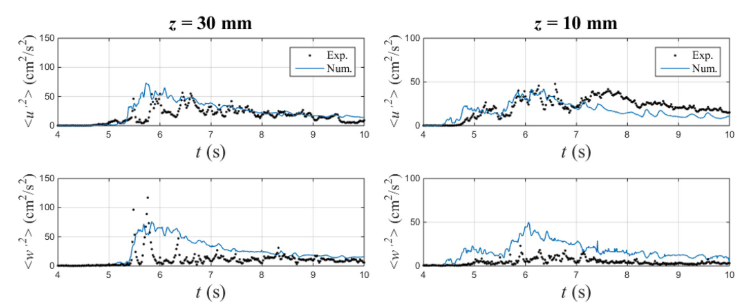
\includegraphics[scale=0.8]{Figures/research_papers/Wang2020-wave-breaking-result.png}
    \caption{Comparisons of numerical and experimental turbulent kinetic energy in x-direction and y-direction. Ref: \parencite{Wang2020}}
    \label{fig:Wang2020-wave-breaking-result}
\end{figure}

Given the model's accuracy, as observed from the figures, the authors conclude that the model's capabilities have been demonstrated, especially in tracking transient-free surfaces. They also reproduce the evolution of turbulence and its intensity due to flow separation. 
However, they note that the model under-predicts the max turbulent kinetic energy and is sensitive to the initial seeding of the turbulent kinetic energy property.
The authors also state that the counteracting effects of the physical viscous dissipation and numerical dissipation, dependent on the particle resolution, would have to be appropriately balanced.
Finally, the authors conclude on the importance of boundary treatment and the need for more sophisticated boundary models to extend the model to $3D$ domains.

%TODO: Need to include Wang2022.

\subsection{LANS-based Models}